\documentclass{standalone}
\usepackage{tikz}

\begin{document}

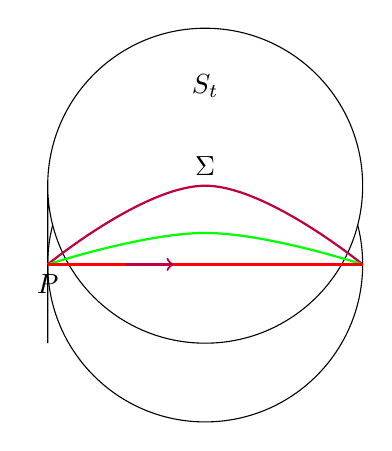
\begin{tikzpicture}[scale=2]
    % Draw the large circle
    \draw (0,0) circle (1);
    
    % Draw the smaller circle inside the large one
    \draw[fill=white] (-1,-0.5) -- (-1,0.5) arc (180:360:1) -- (1,0.5) arc (0:180:1) -- cycle;
    
    % Draw the purple curve
    \draw[thick,purple] plot [smooth,tension=0.7] coordinates {(-1,0) (0,0.5) (1,0)};
    
    % Draw the green curve
    \draw[thick,green] plot [smooth,tension=0.7] coordinates {(-1,0) (0,0.2) (1,0)};
    
    % Draw the red horizontal line
    \draw[red,thick] (-1,0) -- (1,0);
    
    % Label the point P
    \node at (-1,0) [below] {$P$};
    
    % Label the sum symbol
    \node at (0,0.5) [above] {$\Sigma$};
    
    % Label the St
    \node at (0,1) [above] {$S_t$};
    
    % Draw an arrow indicating the direction of the purple curve
    \draw[thick,purple,->] (-0.5,0) -- (-0.2,0);
\end{tikzpicture}

\end{document}